\documentclass[../thesis.tex]{subfiles}
\begin{document}
\chapter{Experimental Results of Standard Algorithms}
\label{ch:experimentsalgos}

Our Python test suite runs all of the algorithms discussed above on a subset of stocks and generates profit figures. The implementation leverages \texttt{Pandas} Dataframes to store and manipulate the stock data. \texttt{Pandas} is a powerful open source data analysis library. See Chapter~\ref{ch:append} for pseudocode of each strategy's implementation. For every buy or sell signal generated in our implementation, the strategies purchased or sold 100 stocks at a time.

To measure the effectiveness of a particular strategy, we use a quality metric to analyze productivity. We compare against a \textit {buy-and-hold} baseline. The baseline measure is created by holding a long position of a specific denomination throughout the entire period of trading. Simply put, shares are bought at the beginning of the period and sold at the end. The profit level is then compared against the performance of the AT strategy. Much of the literature studies the best performance of these strategies over different periods and uses the same baseline comparison \cite{Liu2006} \cite{Aldridge2010} \cite{Garcia2015}. We therefore include the same baseline in this study. However, there are other baseline measures that are implemented in the industry. Some baseline measures compare against mutual fund performances over the trading period. For this baseline method, strategies are often tested against the performance of \texttt{SPY}, a historically high performing fund \cite{Aldridge2010}.

\section{Momentum Strategies}
\label{momentumstrats}

Standalone momentum strategies as a whole very rarely beat out the baseline measure. We tested against a selection of 15 stocks across different industries. Figure~\ref{MOMENTUMfigure}a displays the results of a selection of stocks using SMA, EMA, Bollinger Bands, and RSI: \texttt{AAPL, GOOG, HAS, QCOM,} and \texttt{AMD}. Only a few stocks had performances that beat the baseline. One was \texttt{GOOG}, with both Bollinger Bands and RSI outperforming the baseline profit significantly. \texttt{AMD} for both SMA and EMA proved to be effective as well. However, for most it was more profitable to simply just buy and hold over the period. This performance is counterintuitive, as we should be generating profitable buying and selling trading signals with all of the computation, but that is clearly not the case.  

\begin{figure}[h!]
\centering

\begin{subfigure}[t]{0.9\textwidth}
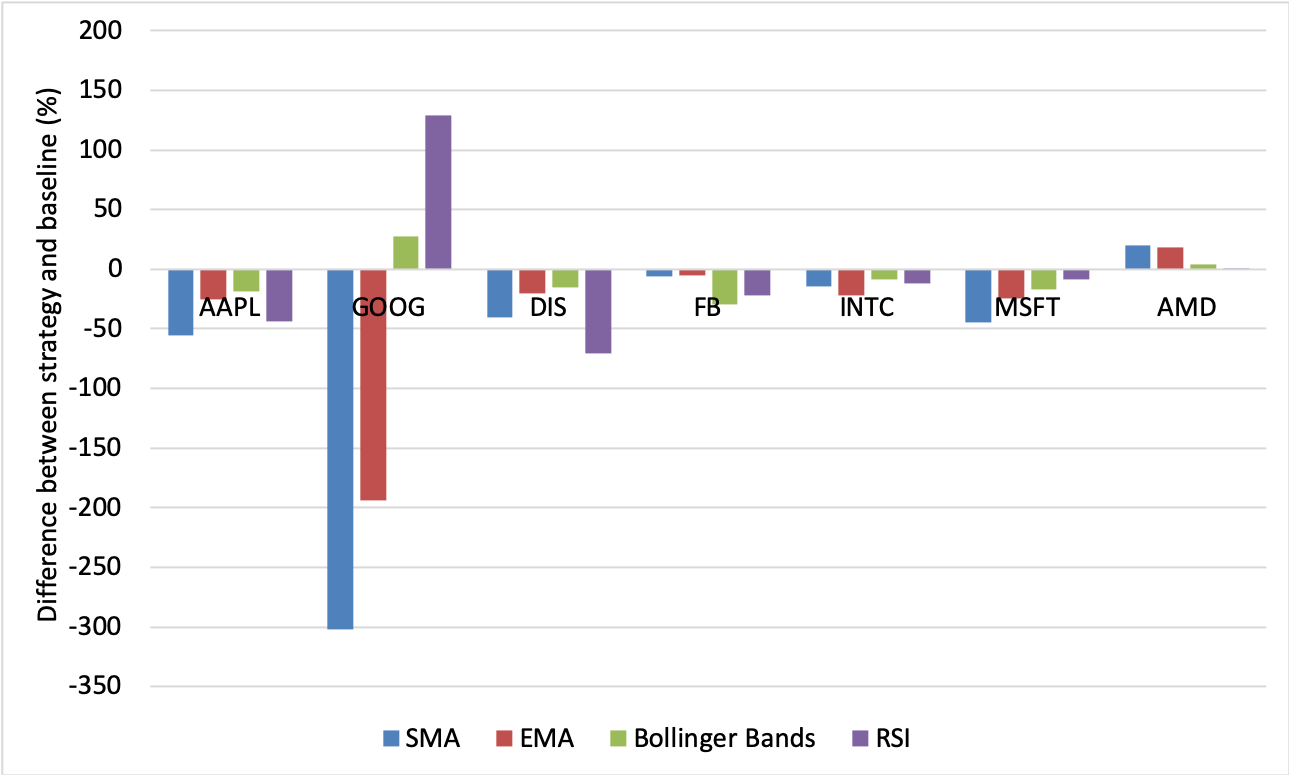
\includegraphics[width=\textwidth]{momentumstrategiesreturns.png}
\caption{Momentum Strategies Individual Results\label{overflow}}
\end{subfigure}
\begin{subfigure}[t]{\textwidth}
\centering 
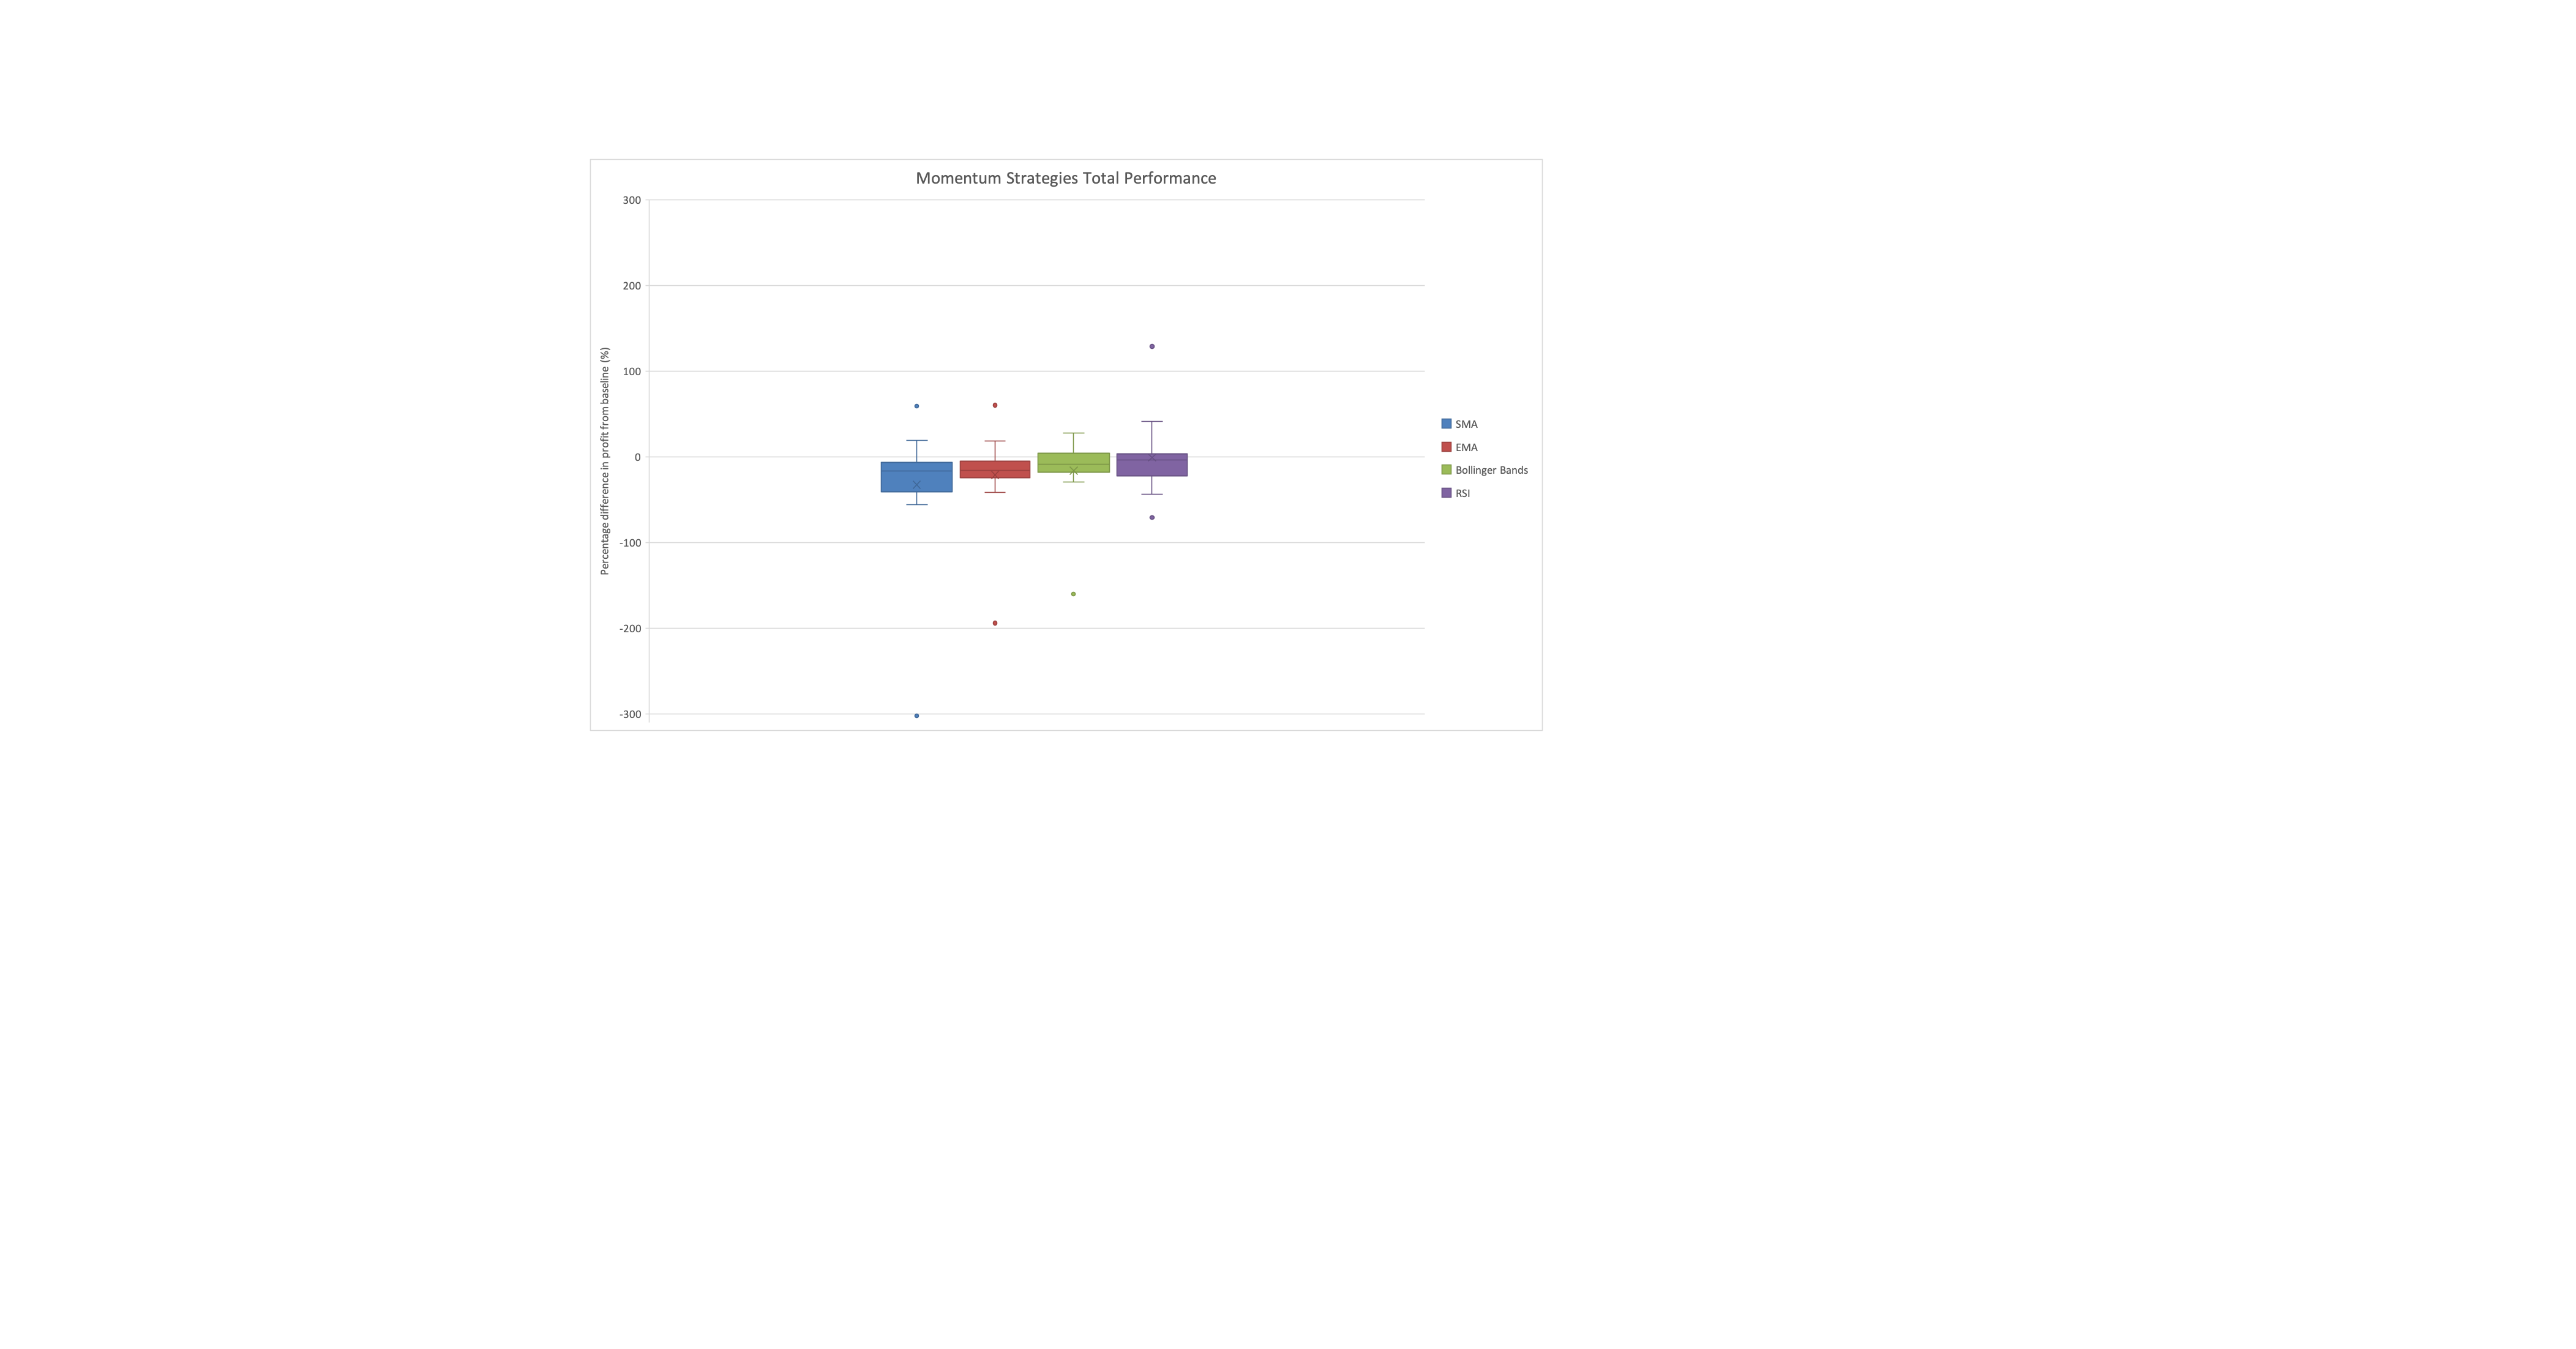
\includegraphics[width=.6\textwidth]{allmomentumstrategies.png}
\caption{ Momentum Strategies Results Across All Stocks \label{overflow}}
\end{subfigure}

\caption{Momentum Strategies Results  \label{overflow}}
\label{MOMENTUMfigure}
\end{figure}


Figure~\ref{MOMENTUMfigure}b shows the performance of each strategy across all 15 stocks tested. We observe that SMA and EMA are the least effective of the strategies, with both of their upper quartiles not even beating the baseline. Bollinger Bands and RSI both have upper quartiles above the baseline, but the median score still doesn't beat the baseline. We observe improved performance as algorithms become more involved and incorporate different statistical measures, but with no median scores outperforming the baseline, we don't observe any success with these strategies. Clearly, these strategies aren't viable as standalone trading algorithms. Now we will discuss why we observed overall poor performance for each algorithm.

The "Golden Cross" strategy when applied to both SMA and EMA isn't particularly effective. Due to the nature of SMA, which generally looks at long periods of time to highlight trends, this can induce a lagged effect to the buy and sell orders. A lagged effect in the context of moving averages is that the current moving average doesn't react to the current trend because of this longer observation window, often making this method ineffective. This lagged effect can be fixed by looking at an EMA analysis \cite{Ehlers}. However, unlike the literature suggests, in practice this doesn't translate to profit. \texttt{AAPL} nearly doubled its profit from using the exponential window that removes the lagged effect yet still had 25.3\% less returns than the baseline. While as a whole the strategy was more effective than SMA and did come closer to baseline performance, it rarely ended up beating it. This suggests that these indicators should be looked at in a different, combined context where multiple indicators could provide more robust trading signals.

With Bollinger Bands, buy and sell signals are still reliant on changes in rolling average prices. However, because of the incorporation of standard deviation, this strategy uses volatility in the market to further base buy and sell decisions. While a significant portion of the chosen stocks didn't end up actually out performing the baseline, a majority of them were within 1-2 percent performance of the baseline. 33\% of stocks tested on the strategy out performed each of its own baseline measure of buying and holding a specific denomination of shares throughout the entire period. Most notably, \texttt{GOOG} outperformed the baseline by 27.7\% while its SMA and EMA performances were an abysmal -302.5\% and -194.1\%, respectively. While still not a passable standalone algorithm, the improvement over SMA and EMA is encouraging.

RSI takes advantage of over-purchasing or overselling of securities to predict convergence back to the mean, taking advantage of mean reversion. Unfortunately, most RSI implementations didn't outperform the baseline. The performance was comparable to Bollinger Bands but slightly improved, as our median performance for this strategy is -3.88\%. While negative, it beats Bollinger Bands median value by over five percentage points. \texttt{GOOG} had by far and away the most impressive performance of any momentum strategy and beat the baseline by 128.8\% while on the other hand \texttt{AAPL} underperformed and posted a -44\% performance compared to the baseline. Overall, our lack of profitable results motivate the need for looking at a more advanced strategy over more fine-grained price data.

%\begin{figure}[h]
%\centering
%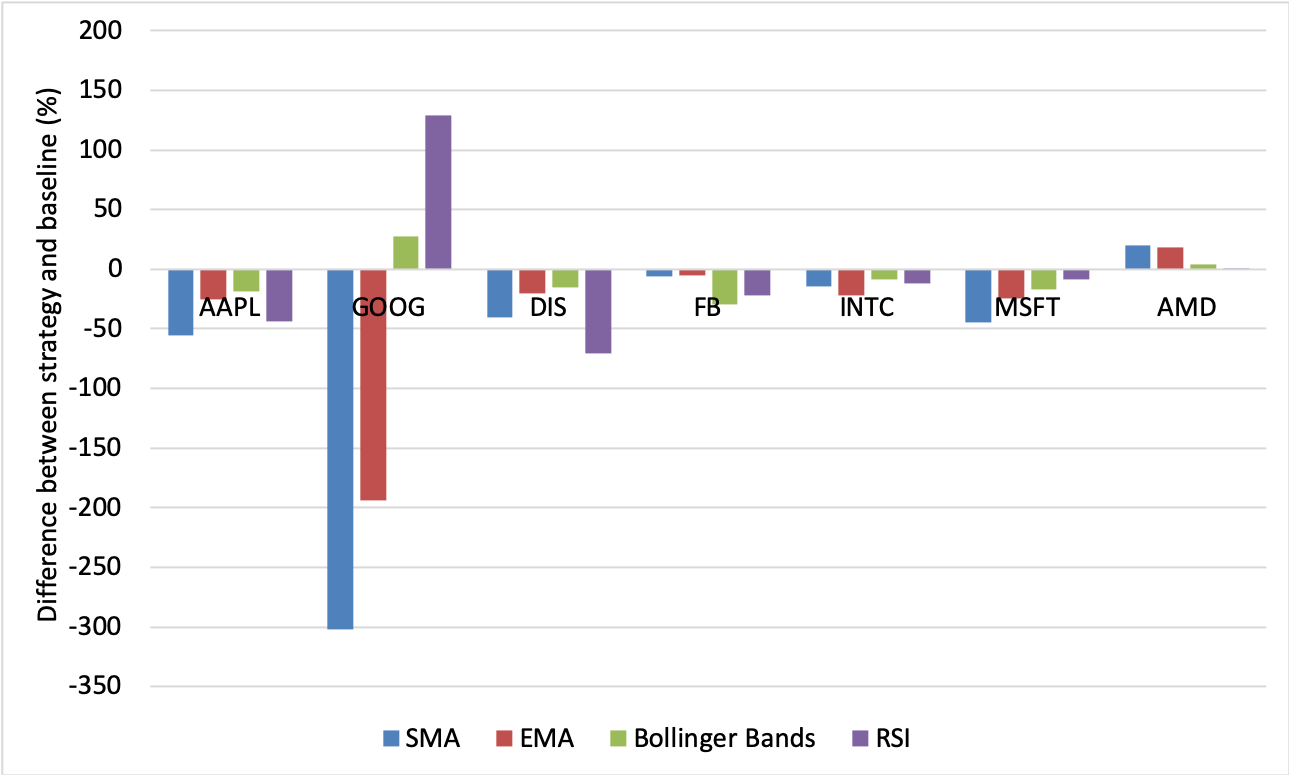
\includegraphics[width=.9\textwidth]{momentumstrategiesreturns.png}
%\caption{Momentum Strategies Results  \label{overflow}}
%\label{MOMENTUMfigur}
%\end{figure}


\section{Combination Momentum Strategies}

The RSI and MACD combined implementation performed incredibly well. Unlike the above section, we use intraday stock data. Our results are from one day of trading on October 26, 2018. Our results were corroborated by choosing a random selection of other days of trading and finding similar results. Of all 29 stocks tested, only 4 stocks ended up with negative profit at the end of the day. Figure~\ref{RSIMACDRESULTSfigure} shows this strong performance. The most notable performances were from \texttt{AAPL} and \texttt{HD}. \texttt{AAPL} out-gained the baseline by 9.07\%  while \texttt{HD} had 4.99\% of profit with the strategy while the baseline lost 3.75\%.  We only observed 27\% of stocks in total that were out-gained by the baseline. \texttt{AXP} is a good example of a poor performing stock - generating a loss of 1.3\% more than the baseline. Across all stocks, we observe the mean performance of this strategy to be 1.18\% and a median performance of 0.23\%. This is a drastic improvement from Section~\ref{momentumstrats}, where all median performances were negative. With enough capital, this strategy could be used to generate incredible returns when using this strategy over multiple days. 

\begin{figure}[h!]
\centering

\begin{subfigure}[t]{0.74\textwidth}
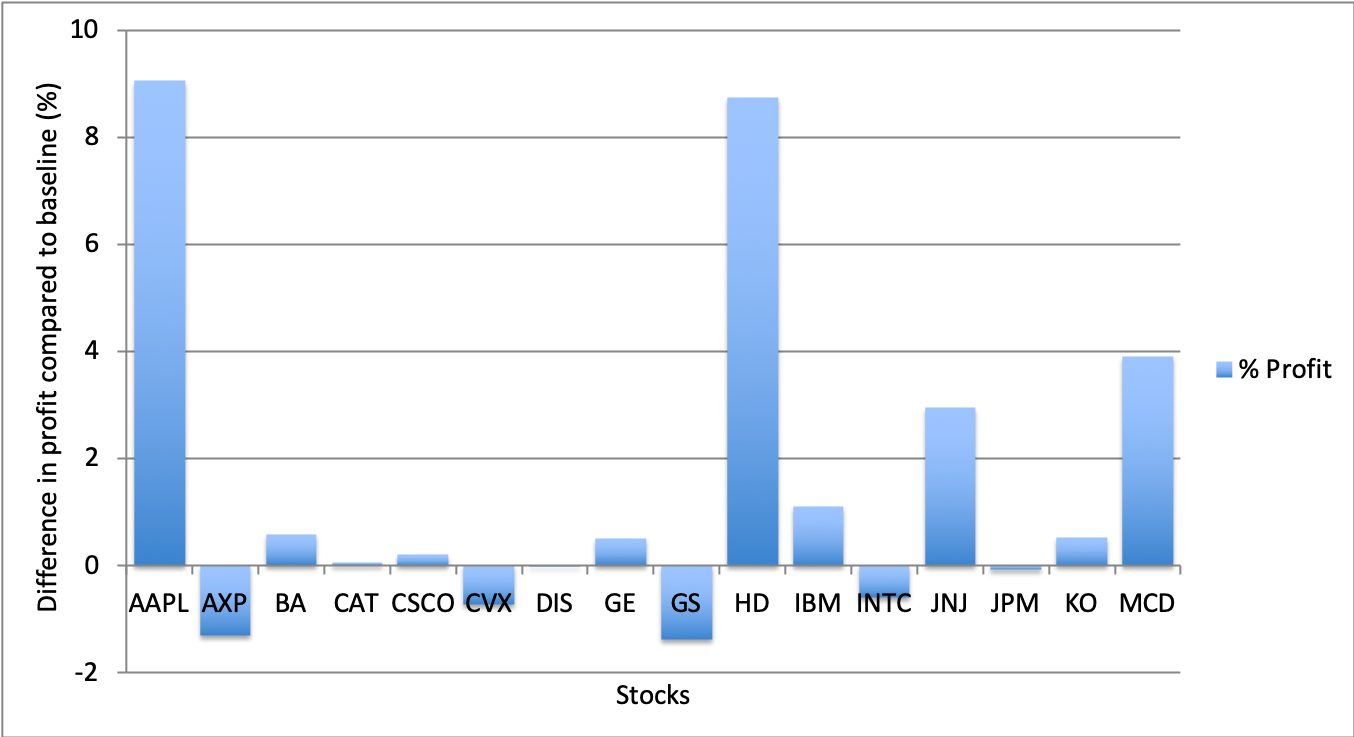
\includegraphics[width=\textwidth]{rsimacdresults.png}
\caption{RSI/MACD Individual Results\label{overflow}}
\end{subfigure}
\begin{subfigure}[t]{.215\textwidth}
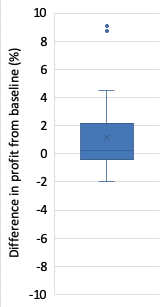
\includegraphics[width=\textwidth]{allrsimacdstrat.png}
\caption{ Total Results \label{overflow}}
\end{subfigure}

\caption{RSI/MACD Strategy Results  \label{overflow}}
\label{RSIMACDRESULTSfigure}
\end{figure}

This algorithm generates incredibly robust buy signals and frequent sell signals which can nearly guarantee gains after buy signals. Therefore, having millions of dollars of existing capital and allowing us to purchase higher denominations of shares of a given stock can generate even more profits with less risk of massive losses. However, rather than focusing on individual stocks over time, this combination strategy is best implemented over a pool of multiple stocks because it isn't uncommon for days to generate absolutely zero buy signals for a given stock. Unfortunately, the barrier to entry for individuals to generate these massive profits is being able to access up to the second stock data, which requires requires tens of thousands of dollars per year \cite{Treleaven2013}. All data found via the internet or Quandl is delayed by upwards of 20 minutes, which can make the difference between thousands of dollars and profits and thousands of dollars of losses.

%\begin{figure}[h]
%\centering
%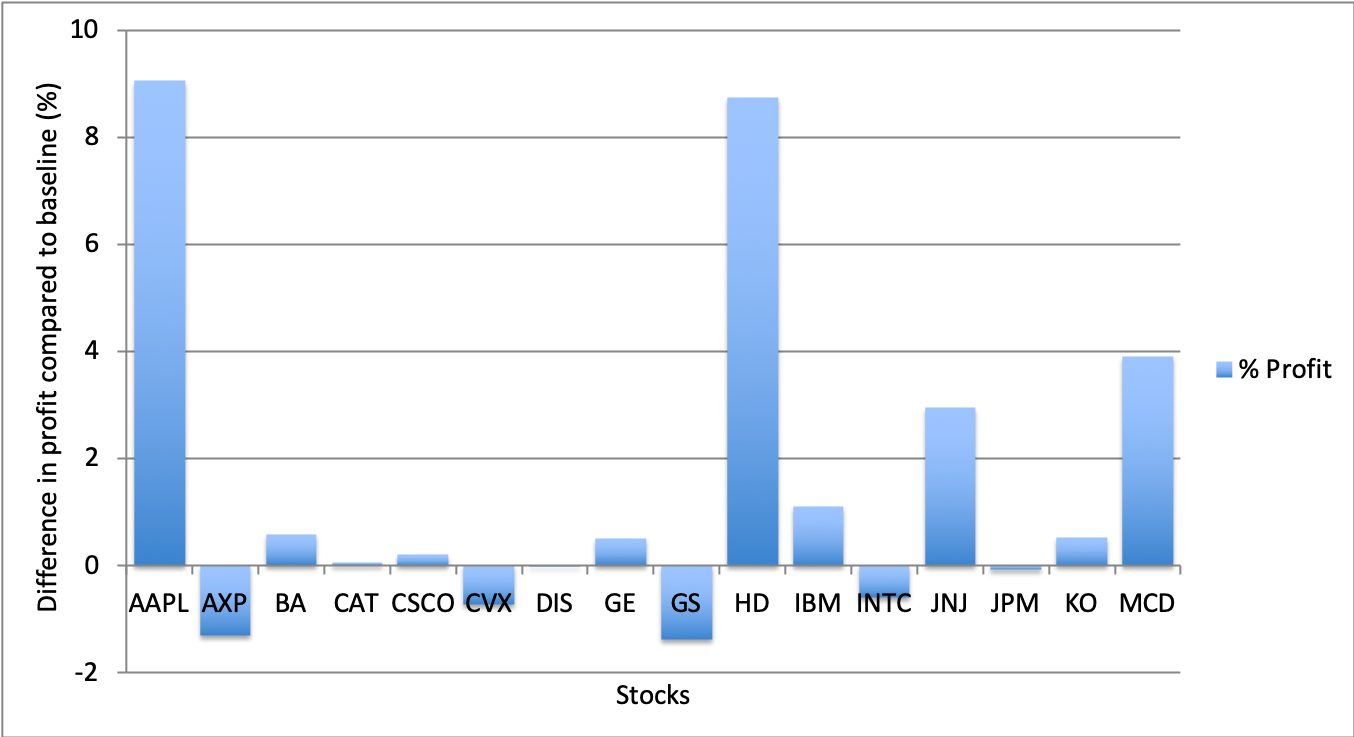
\includegraphics[width=.9\textwidth]{rsimacdresults.png}
%\caption{RSI and MACD strategy   \label{overflow}}
%\label{RSIMACDRESULTSfigure}
%\end{figure} 



\section{Pairs Trading}

Just like our combined momentum strategy, our pairs trading implementation performed incredibly well. Because we are trading two different stocks in this method, we \textit{buy-and-hold} both stocks over the trading period. However, we only found 5 combinations of stocks that were cointegrated enough to conisder trading. When the cointegration p-values of a pair of stocks is less than .05, this signals cointegration at a 95\% confidence level \cite{Gatev2006}. Further study would identify more pairs of cointegrated stocks from a larger pool of stocks. When trading \texttt{AMD} with \texttt{SBUX}, the strategy profited 205.89\% over the baseline. \texttt{QCOM} and \texttt{SBUX} also found success - culminating in 122.37\% returns over the baseline. However, even the lowest performing combination, \texttt{AMD} and \texttt{VOD}, beat out the baseline by over 32.4\%. Figure~\ref{PAIRSRESULTSfigure} shows these truly astounding results. 

\begin{figure}[h]
\centering
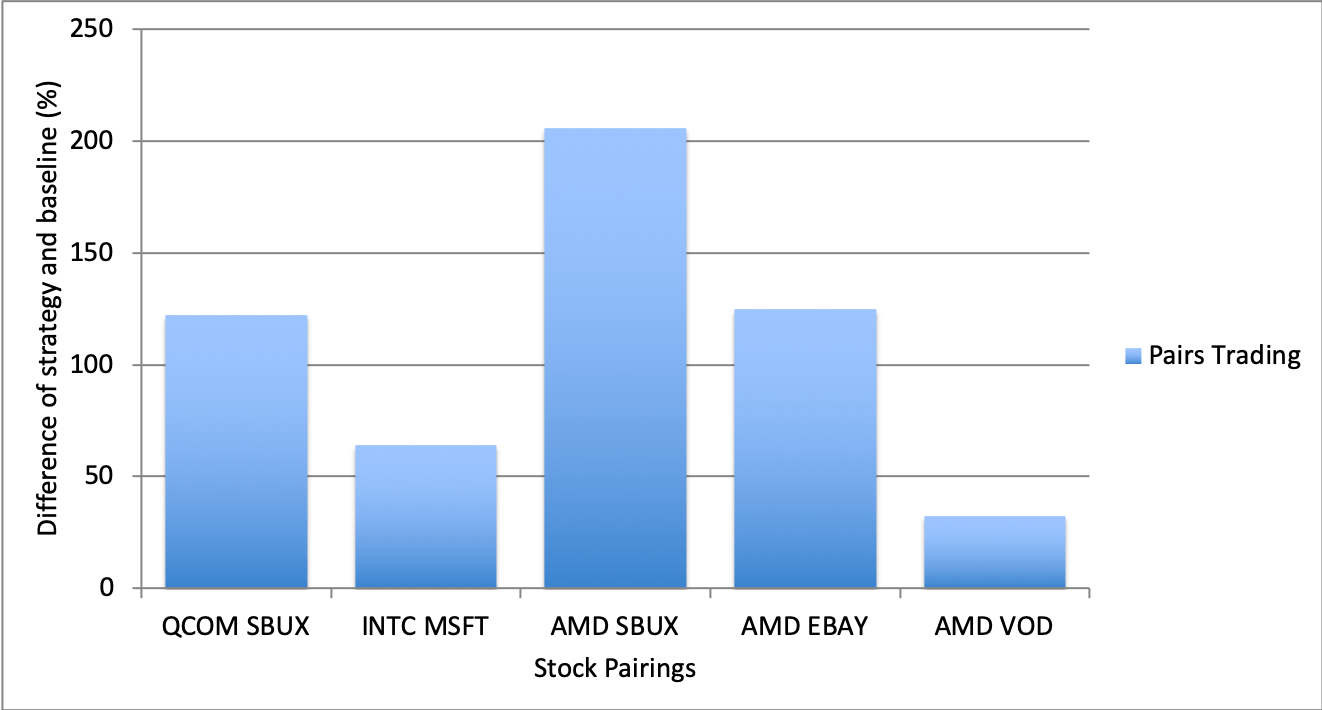
\includegraphics[width=.77\textwidth]{pairstradingresults.png}
\caption{Pairs Trading Results \label{overflow}}
\label{PAIRSRESULTSfigure}
\end{figure}

This highlights a common trend. More involved strategies that use multiple measures or inputs always perform better than single measures and nearly always beat the baseline. Both the combined RSI/MACD and pairs trading strategies were very successful. Using these strategies, someone could make incredible profits. However it is important to acknowledge limitations as well. For all of our algorithms studied in this section, we only test a very small subset of the larger DJIA. Future studies would look to include many more stocks to better understand the effectiveness of these strategies. 

\end{document}
